\subsubsection{Objetos de Transferencia de datos (DTO)}
Por última parte, en las figuras , tenemos a las clases DTO. Estas clases, como se mencionó anteriormente, son utilizadas por las clases de tipo repositorio, servicio y controlador, por lo que son una pieza clave dentro del proyecto.


\begin{figure}[htbp!]
	\begin{center}
		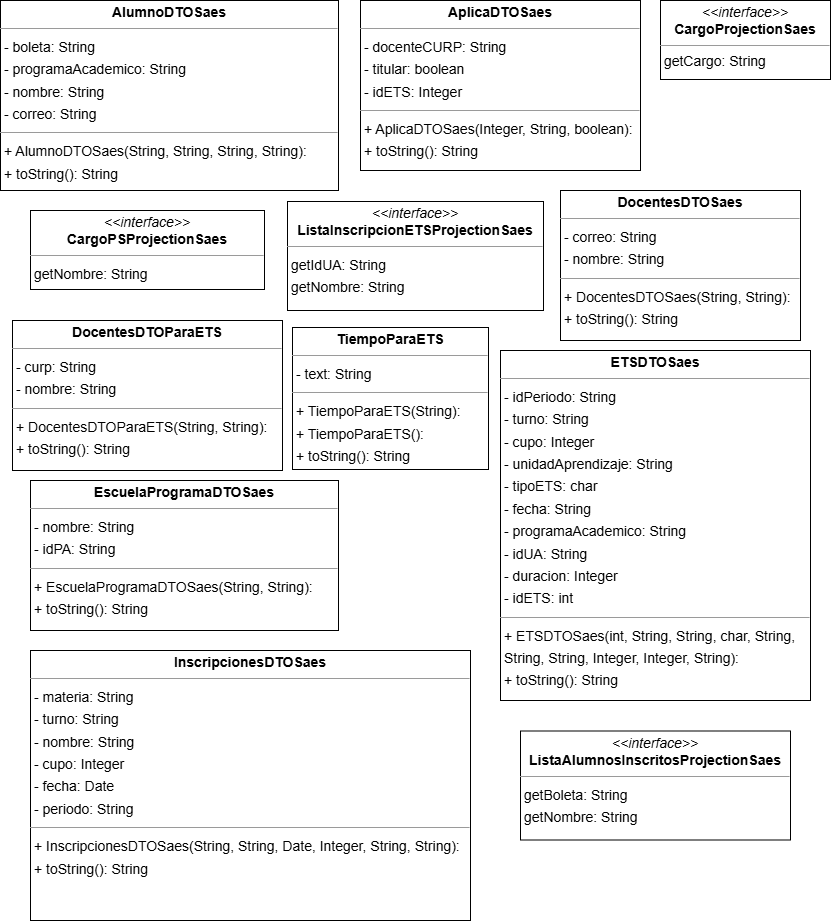
\includegraphics[width=0.85\textwidth]{Clases/DTO1.png}
		\caption{Diagrama de clases de los DTO del servidor parte 1.}
		\label{fig:DTO1}
	\end{center}
\end{figure}

\begin{figure}[htbp!]
	\begin{center}
		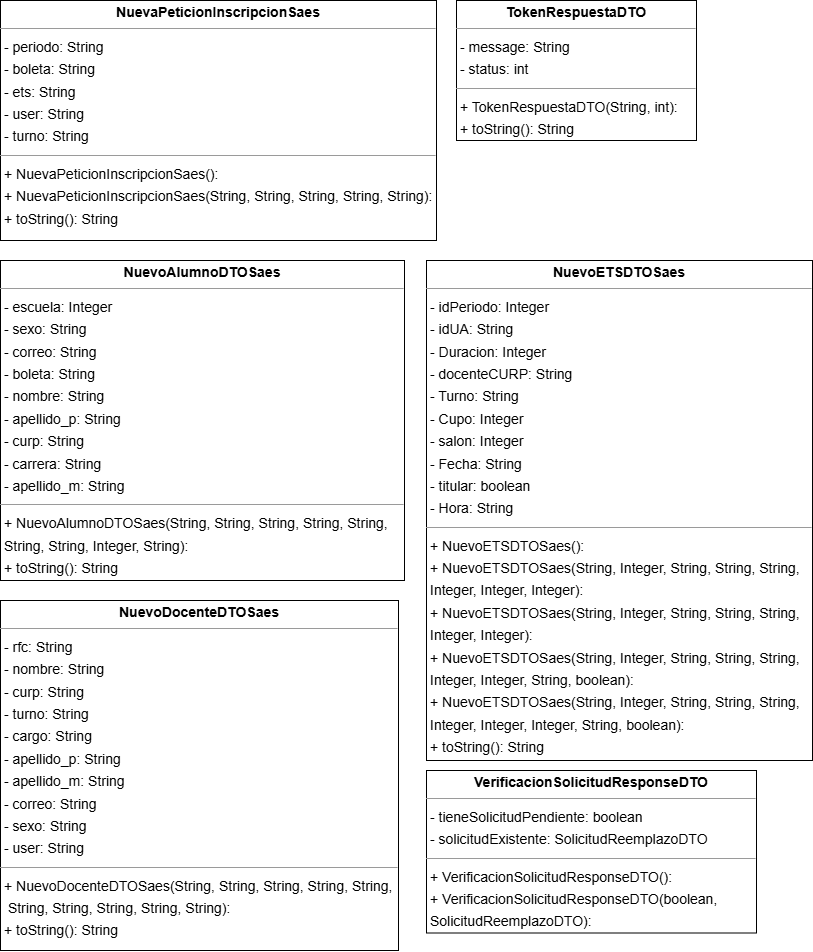
\includegraphics[width=0.9\textwidth]{Clases/DTO2.png}
		\caption{Diagrama de clases de los DTO del servidor parte 2.}
		\label{fig:DTO2}
	\end{center}
\end{figure}

\begin{figure}[htbp!]
	\begin{center}
		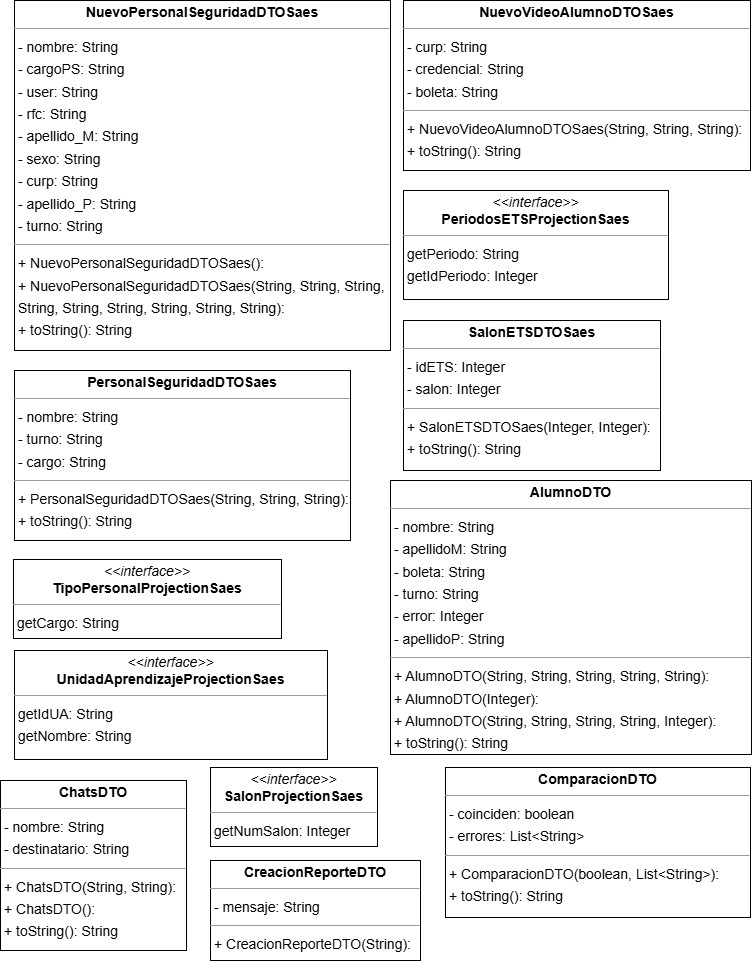
\includegraphics[width=0.9\textwidth]{Clases/DTO3.png}
		\caption{Diagrama de clases de los DTO del servidor parte 3.}
		\label{fig:DTO3}
	\end{center}
\end{figure}

\begin{figure}[htbp!]
	\begin{center}
		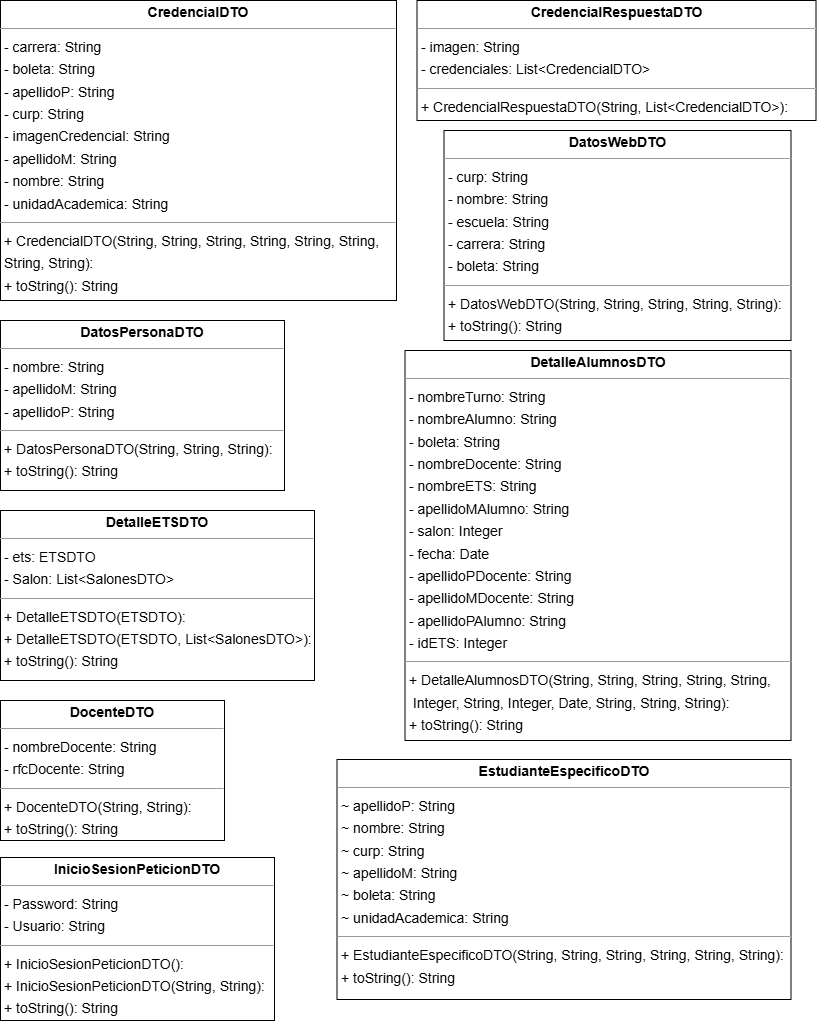
\includegraphics[width=0.9\textwidth]{Clases/DTO4.png}
		\caption{Diagrama de clases de los DTO del servidor parte 4.}
		\label{fig:DTO4}
	\end{center}
\end{figure}

\begin{figure}[htbp!]
	\begin{center}
		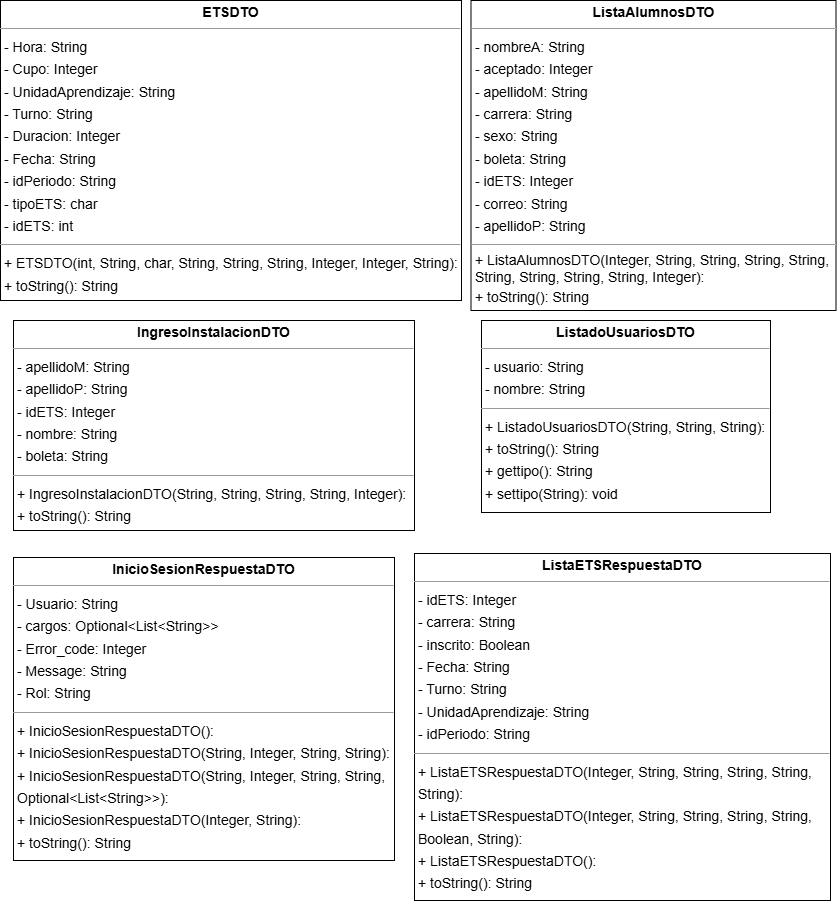
\includegraphics[width=0.9\textwidth]{Clases/DTO5.png}
		\caption{Diagrama de clases de los DTO del servidor parte 5.}
		\label{fig:DTO5}
	\end{center}
\end{figure}

\begin{figure}[htbp!]
	\begin{center}
		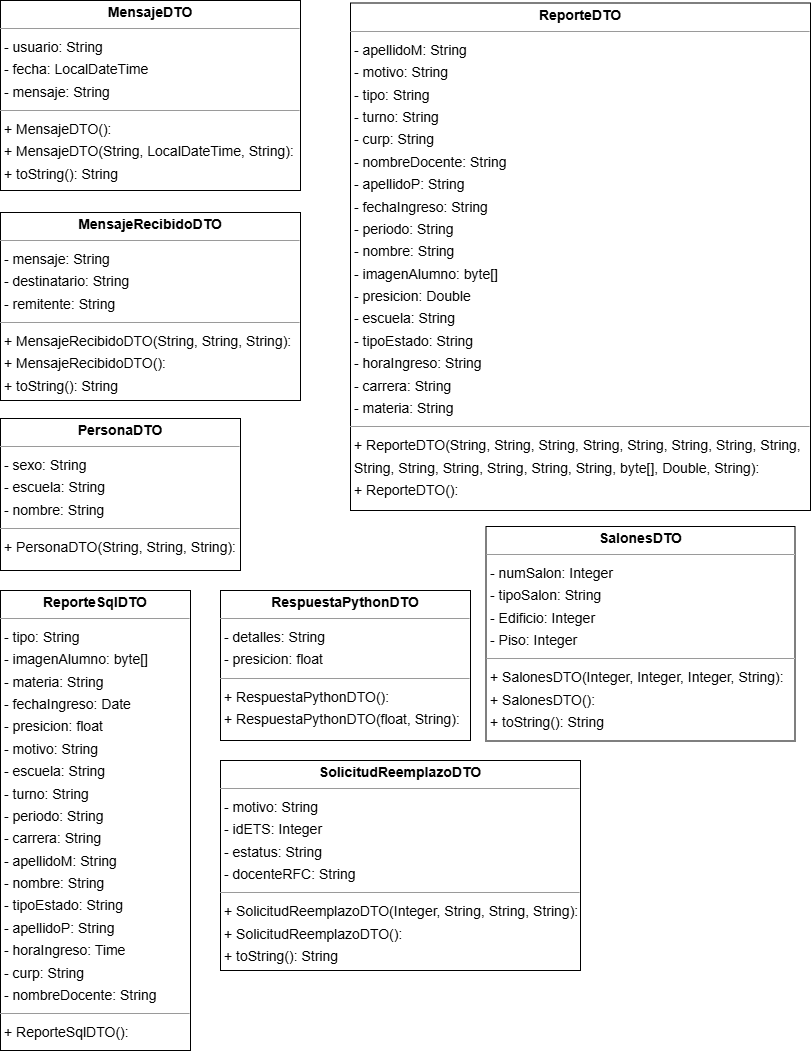
\includegraphics[width=0.9\textwidth]{Clases/DTO6.png}
		\caption{Diagrama de clases de los DTO del servidor parte 6.}
		\label{fig:DTO6}
	\end{center}
\end{figure}